\documentclass[11pt]{beamer}
\usetheme{UMONS}
\usepackage[utf8]{inputenc}
\usepackage[english]{babel}
\usepackage{amsmath}
\usepackage{amsfonts}
\usepackage{amssymb}
\usepackage{graphicx}
\usepackage{color}
\usepackage{marvosym}
\author{Sébastien Gamrath}
\title{Paradoxe de Zénon}
%\setbeamercovered{transparent} 
%\setbeamertemplate{navigation symbols}[vertical] 
%\logo{UMONS} 
\begin{document}
\begin{frame}{Paradoxe de Zénon}
	\pause Ou la fable du lièvre et de la tortue par Zénon d'\'{E}lée en 450 ACN
	\vspace{0.5cm}
	\pause \\ \color{umons-red} \textbf{\'{E}noncé du} \textit{paradoxe}
	\pause \\ \color{black}Le paradoxe d'Achille et de la tortue tel que formulé par Zénon dit qu'un jour, Achille, le héros grec, disputa une course avec une tortue. Achille étant un athlète de bon niveau et étant bon joueur, il laisse un avance à la tortue. \pause Zénon affirme qu'il ne pourra jamais rattraper le lent reptile. En effet, bien qu'Achille court beaucoup plus vite, le temps qu'il parcourt la distance qu'il a laissé à la tortue, cette dernière a parcouru une certaine distance non nulle donc elle a encore de l'avance. Le temps qu'Achille rattrape ce retard, la tortue a encore avancé et le processus est itéré. Achille ne rattrape donc jamais la tortue.
\end{frame}
\begin{frame}{Paradoxe de Zénon}
	Peut-être sera-ce plus clair sur cette figure : 
	\begin{center}
		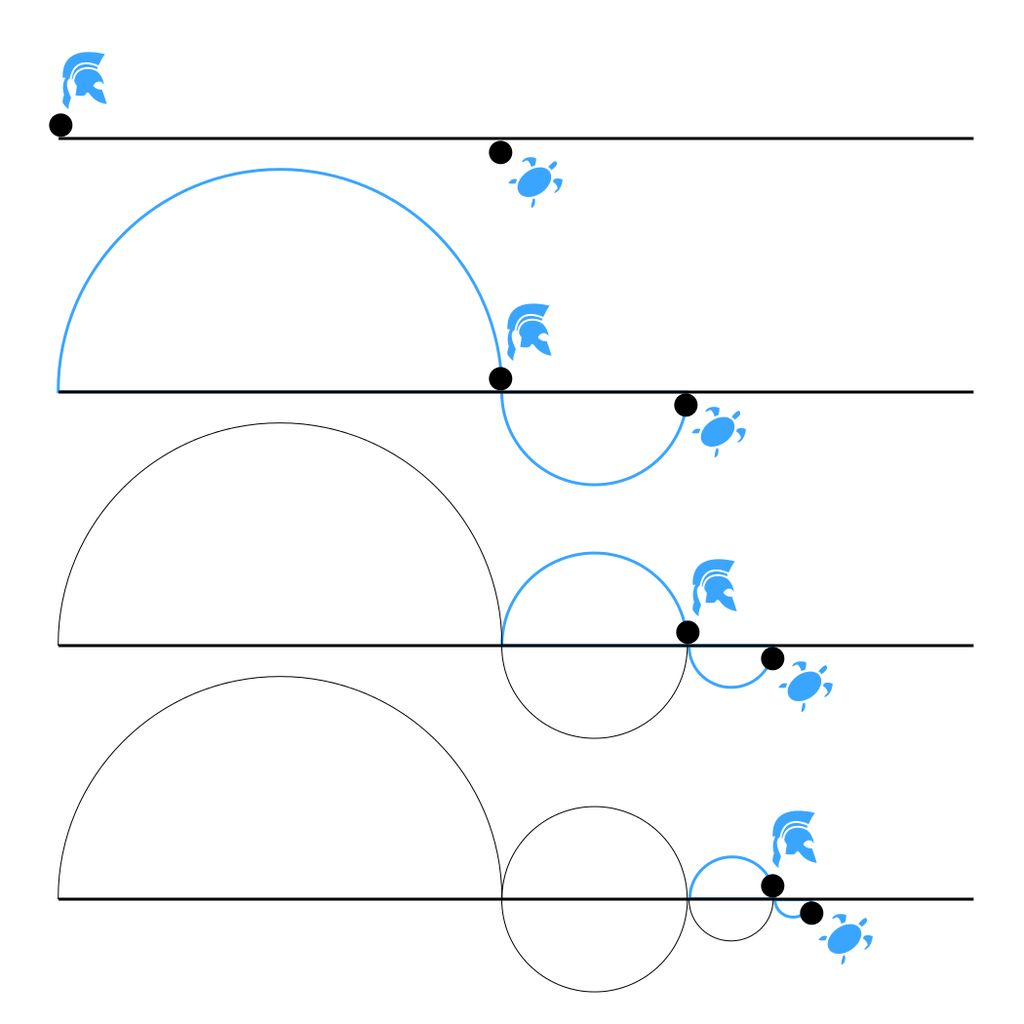
\includegraphics[scale=0.2]{ZAPT1.png}
	\end{center}
\end{frame}
\begin{frame}{Paradoxe de Zénon}
Une autre manière de voir le paradoxe
\begin{center}
	
\includegraphics[scale=0.5]{glass1.png}
\end{center}
\end{frame}
\begin{frame}{Paradoxe de Zénon}
Une autre manière de voir le paradoxe
\begin{center}
	
\includegraphics[scale=0.5]{glass2.png}
\end{center}
\end{frame}
\begin{frame}{Paradoxe de Zénon}
Une autre manière de voir le paradoxe
\begin{center}
	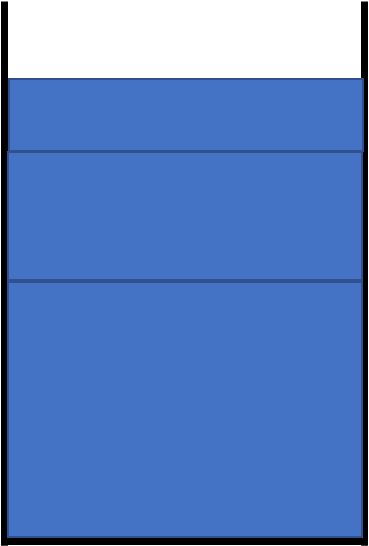
\includegraphics[scale=0.5]{glass3.png}
\end{center}
\end{frame}
\begin{frame}{Paradoxe de Zénon}
Une autre manière de voir le paradoxe
\begin{center}
	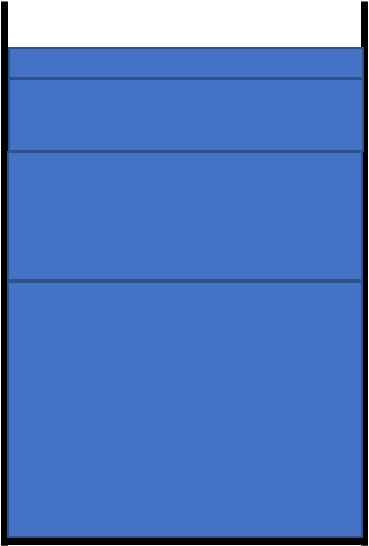
\includegraphics[scale=0.5]{glass4.png}
\end{center}
\end{frame}
\begin{frame}{Paradoxe de Zénon}
Une autre manière de voir le paradoxe
\begin{center}
	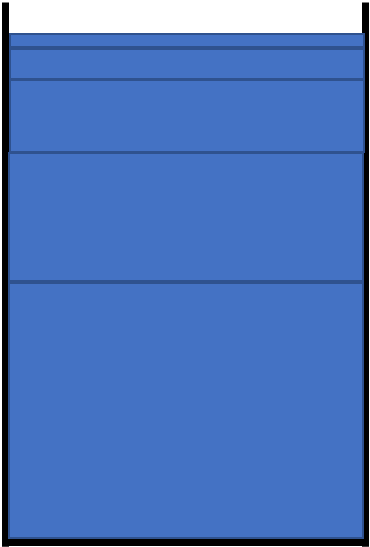
\includegraphics[scale=0.5]{glass5.png}
\end{center}
\end{frame}
\begin{frame}{Paradoxe de Zénon}
Retour à la course entre Achille et la tortue 
\pause
\begin{center}
	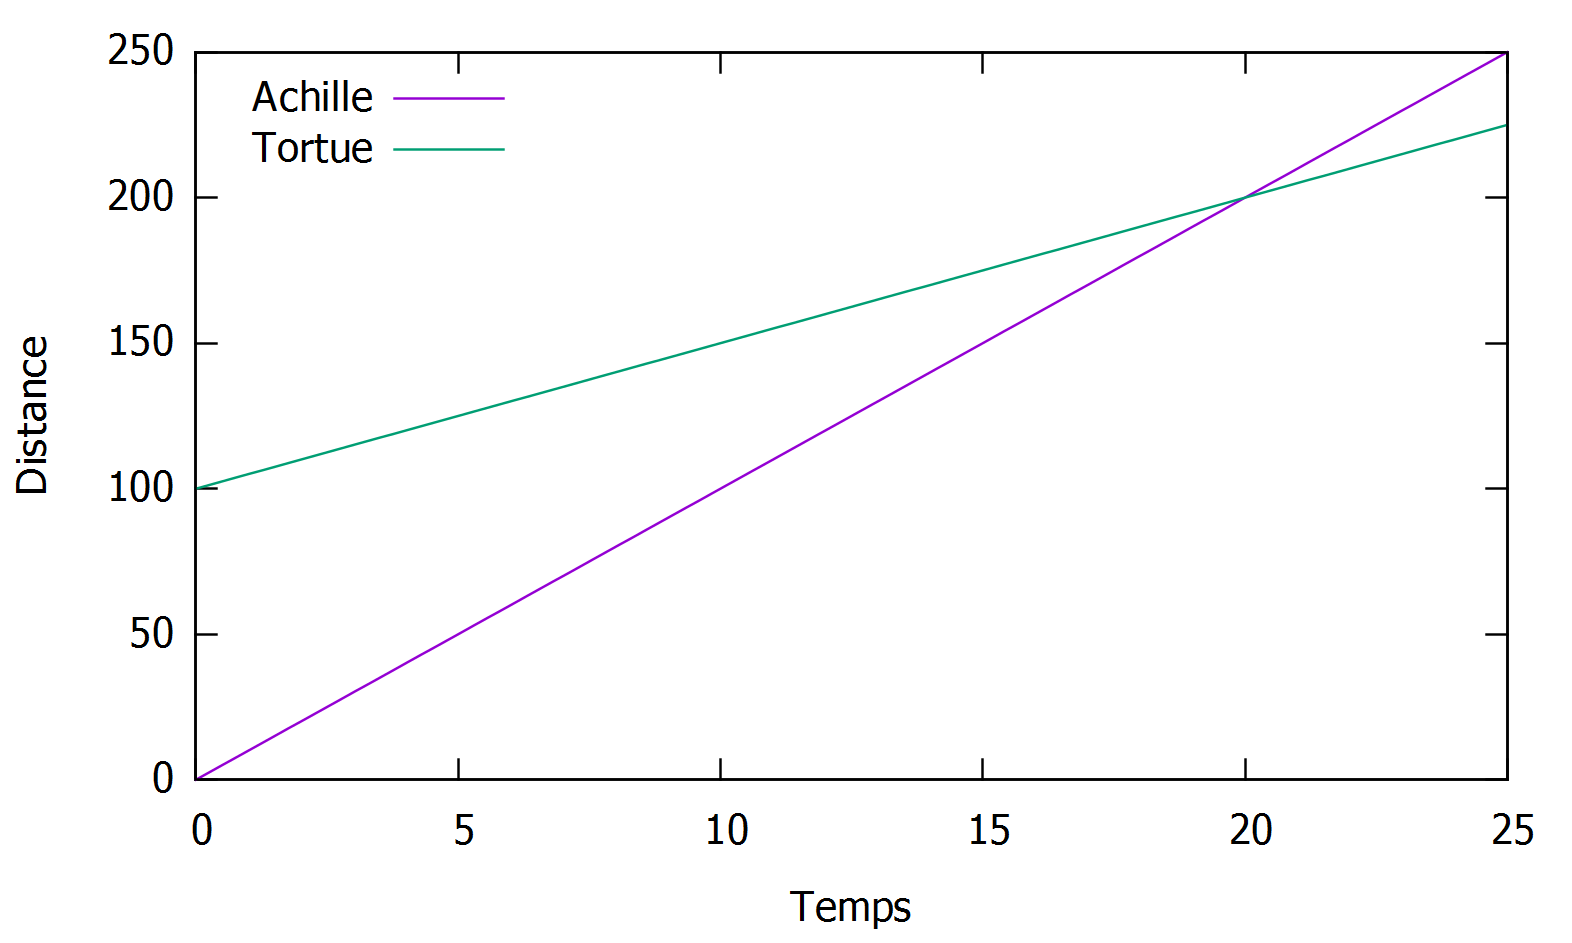
\includegraphics[scale=0.35]{ZAPT2.png}
\end{center}
\end{frame}
\begin{frame}{Paradoxe de Zénon}
	Séries convergentes :
	\\ Si Achille se déplace à 10 m/s et la tortue à 5 m/s et qu'initialement la distance entre les deux vaut 100m, alors on a à résoudre : 
	\[ T = 10 + 5 + 2.5 + 1.25 + ...\] \pause
	Autrement dit :
	\[ \sum_{n=1}^{\infty} \frac{10}{2^n}\]
	C'est la somme d'une série géométrique : \[\sum_{k=1}^{\infty} ax^k = \frac{a}{1-x} \] \pause 
	Donc dans notre cas : \[ T = \frac{10}{1- 0.5} = 20 \]
\end{frame}
\end{document}